\documentclass[12pt,letterpaper,titlepage,en-US]{article}

\usepackage{basicstyle}
\usepackage{report}
%
% Homework Details
%   - Title
%   - Due date
%   - Class
%   - Section/Time
%   - Instructor
%   - Author
%

\newcommand{\hmwkTitle}{Health/Fitness Program}
\DTMsavetimestamp{DueDate}{2016-12-7T23:59:59-06:00}
\newcommand{\hmwkClass}{CS 6360.003}
\newcommand{\hmwkClassName}{Database Design}
\newcommand{\hmwkClassInstructor}{Instructor: Nurcan Yuruk}
\newcommand{\hmwkAuthorName}{Hanlin He / Kai Kang}
\newcommand{\hmwkAuthorNetID}{hxh160630 / kxk151230}


%
% Title Page
%

\title{
    \vspace{2in}
    \textmd{\textbf{\hmwkClassName \\\hmwkClass:\ \hmwkTitle }}\\
    \normalsize\vspace{0.1in}\small{Due\ on\ \DTMusedate{DueDate}\ at \DTMusetime{DueDate} }\\
    \vspace{0.1in}\large{\textit{\hmwkClassInstructor}}
    \vspace{3in}
}

\author{\textbf{\hmwkAuthorName\ \footnotesize{(\hmwkAuthorNetID)}} \\ }
\date{}
\makeindex

\begin{document}
\maketitle

\pagenumbering{Roman}

\tableofcontents

\pagebreak
\pagenumbering{arabic}


% Requirements collection: comprehensive, detail-oriented system (20 points)
% ER/EER (20 points)
% Mapping to relational model and normalization (20 points)
% SQL (10 points)
% PL/SQL (30 points)

\section{Requirement}
The Fitness System’s main purpose is to assist the UT Dallas Fitness Center management. Management mainly care about these aspects: customer management, fitness program management, equipment management, and sport session management. The system shall include the following function and features.
\begin{enumerate}
    \item The system shall keep track of customer’s profile. Basic information shall include name, address, phone, age, sexuality, height, weight. Each customer should have a customer id for identification. Each customer should have a membership id(valid date and expiration date) and a closet.
    \item The system shall provide multiple fitness programs at different difficulty levels. The fitness program shall have the following information: name, type (aerobic/strength/HIIT), list of equipment needed. For aerobic training, additional informations about the exercise intensity and minimal exercise time shall be available. In particular, there are four types of aerobic: treadmill, elliptical, exercise bike and rowing machine.
    \item The system shall keep information about employees. Employees include trainer, equipment maintainer. Each trainer is eligible for some training programs.
    \item Customer need to sign a contract to exercise in the Fitness Center. In the contract, customer can choose a fitness program. The system shall record the contract No.
    \item The system shall keep information about all equipments, including name, price, vendor, model and age. each equipment's price can be implied by its vendor and model to identify.
    \item Each equipment shall have one maintainer responsible for maintenance.
    \item The system shall track and store the exercise sessions data for all customer, include exercise type, exercise session duration, average heart rate, maximum heart rate, estimate calories burnt. For aerobic training, types, distance and average pace shall be stored.
    \item The system shall support occasional deal event, such as add bonus time for member registered during a specific period.
    \item The system shall support clean up the exercise session data for long time idle user.
\end{enumerate}

\pagebreak
\section{Enhanced Entity-Relation Diagram}
The EER is shown in \cref{eer}.

\begin{figure}[H]
    \caption{EER for Fitness Program}\label{eer}
    \centering
    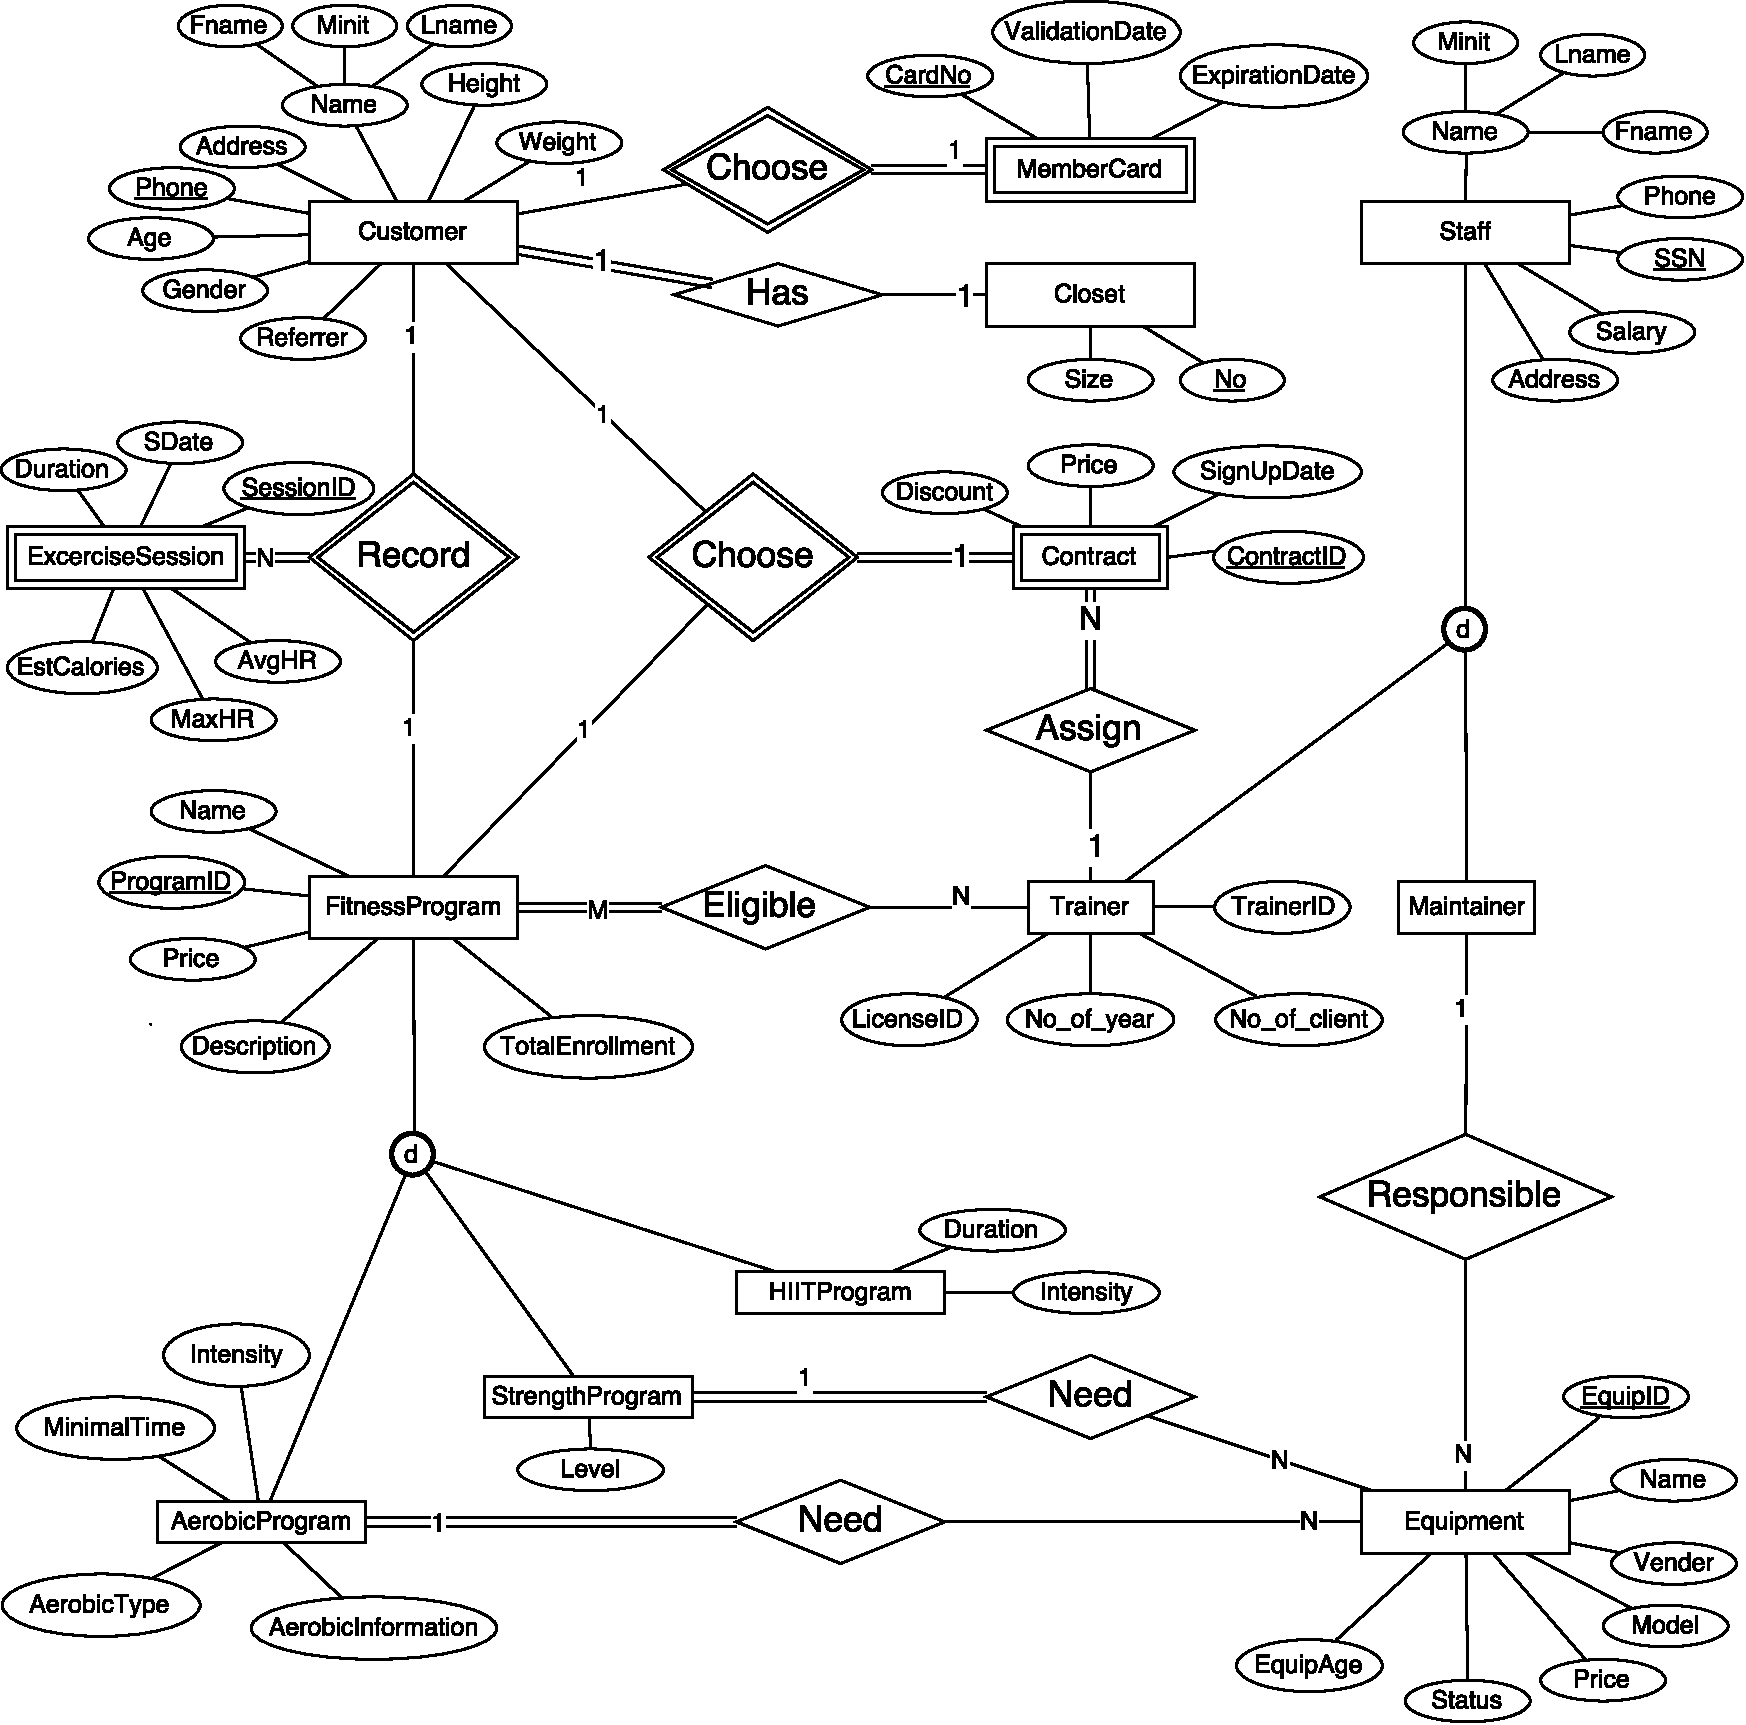
\includegraphics[width=\textwidth]{img/eer}
\end{figure}

\pagebreak
\section{Mapping EER Diagram to Relational Schema and Normalization}
The relational schema mapped from EER is shown in\cref{sdam}.

\begin{figure}[H]
    \caption{Relational Schema after Mapping}\label{sdam}
    \centering
    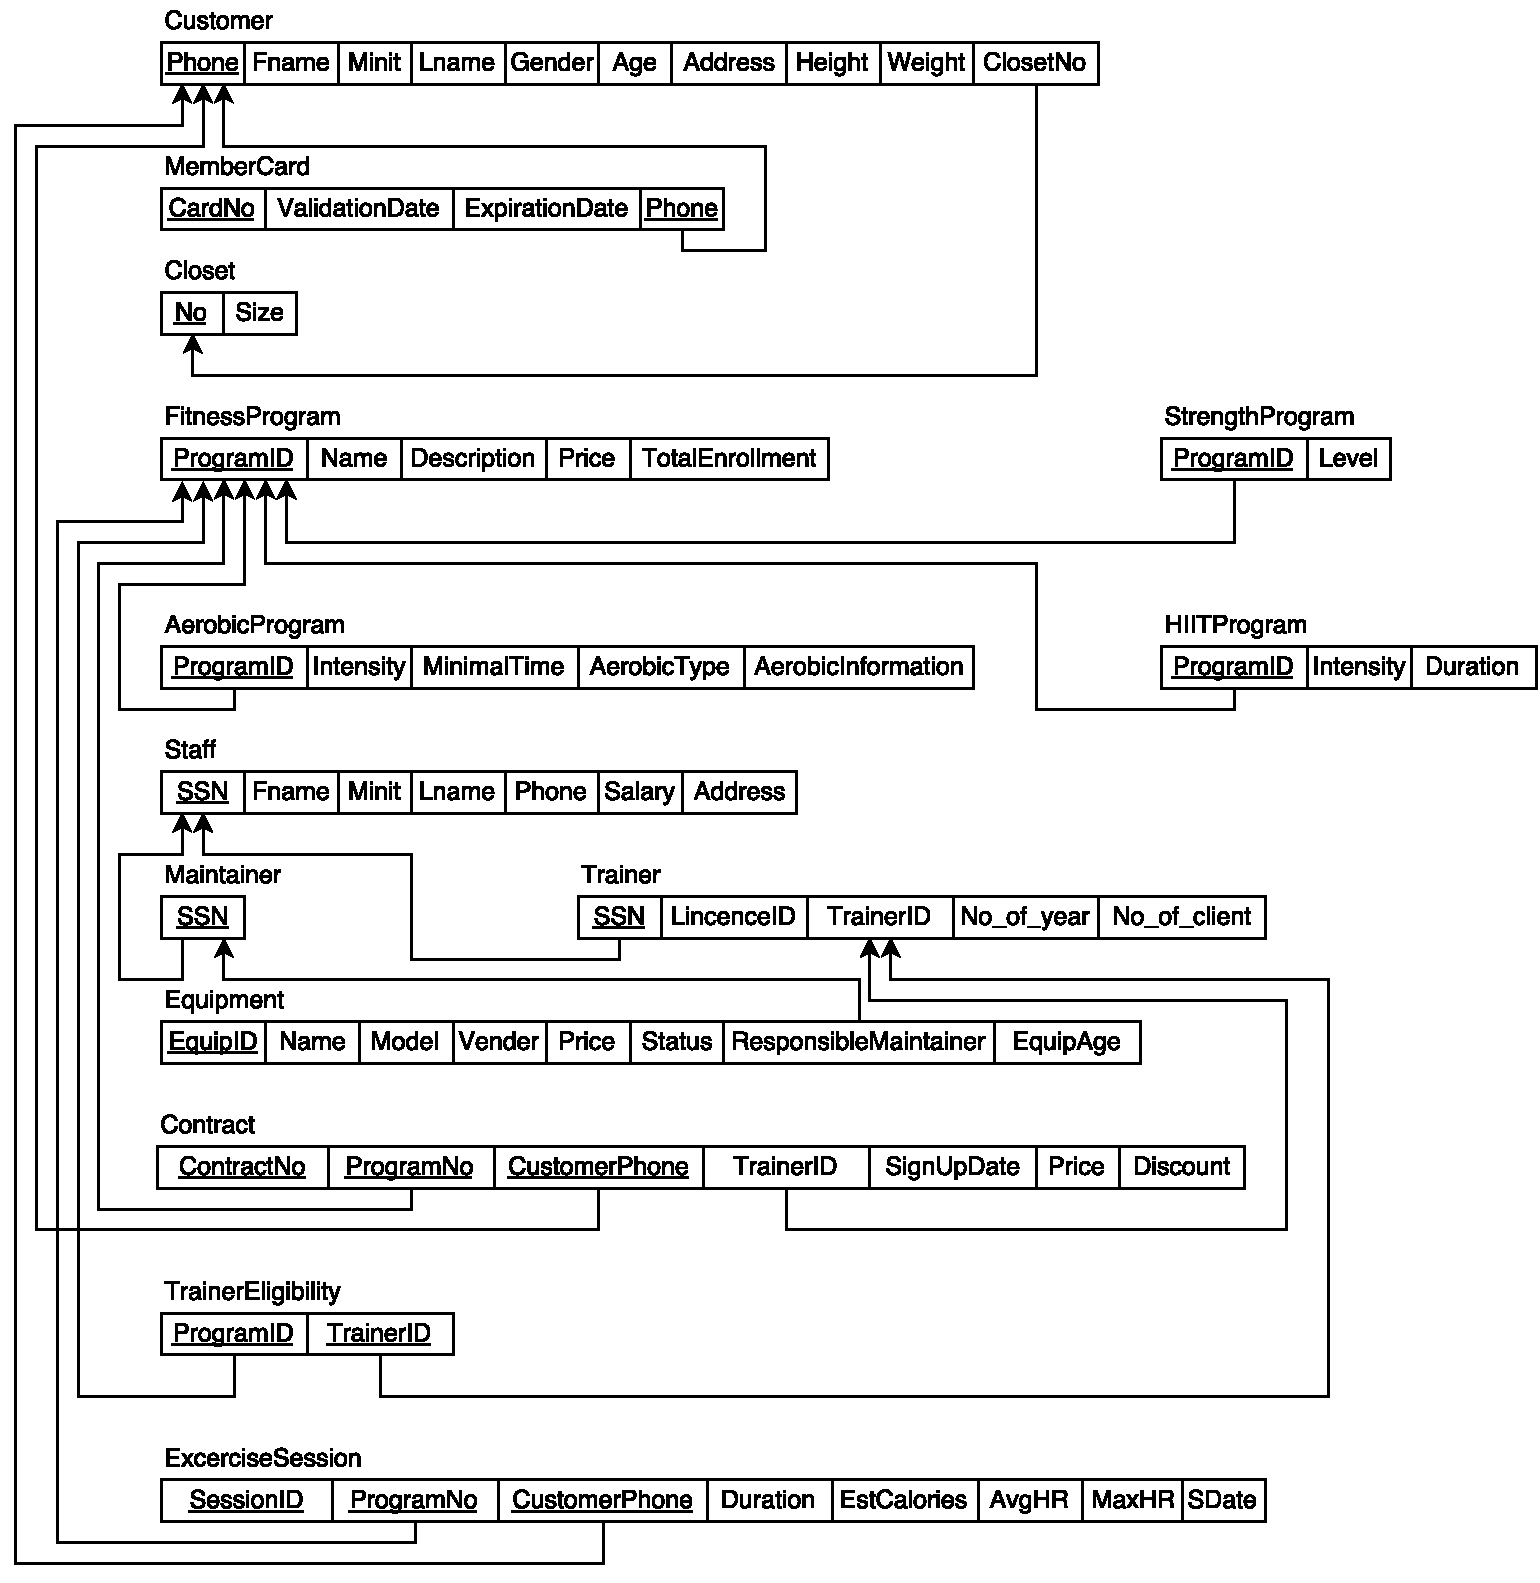
\includegraphics[width=\textwidth]{img/sdam}
\end{figure}

\pagebreak
The functional dependencies in the schema is shown in \cref{fd}.
\begin{figure}[H]
    \caption{Original Functional Dependencies}\label{fd}
    \centering
    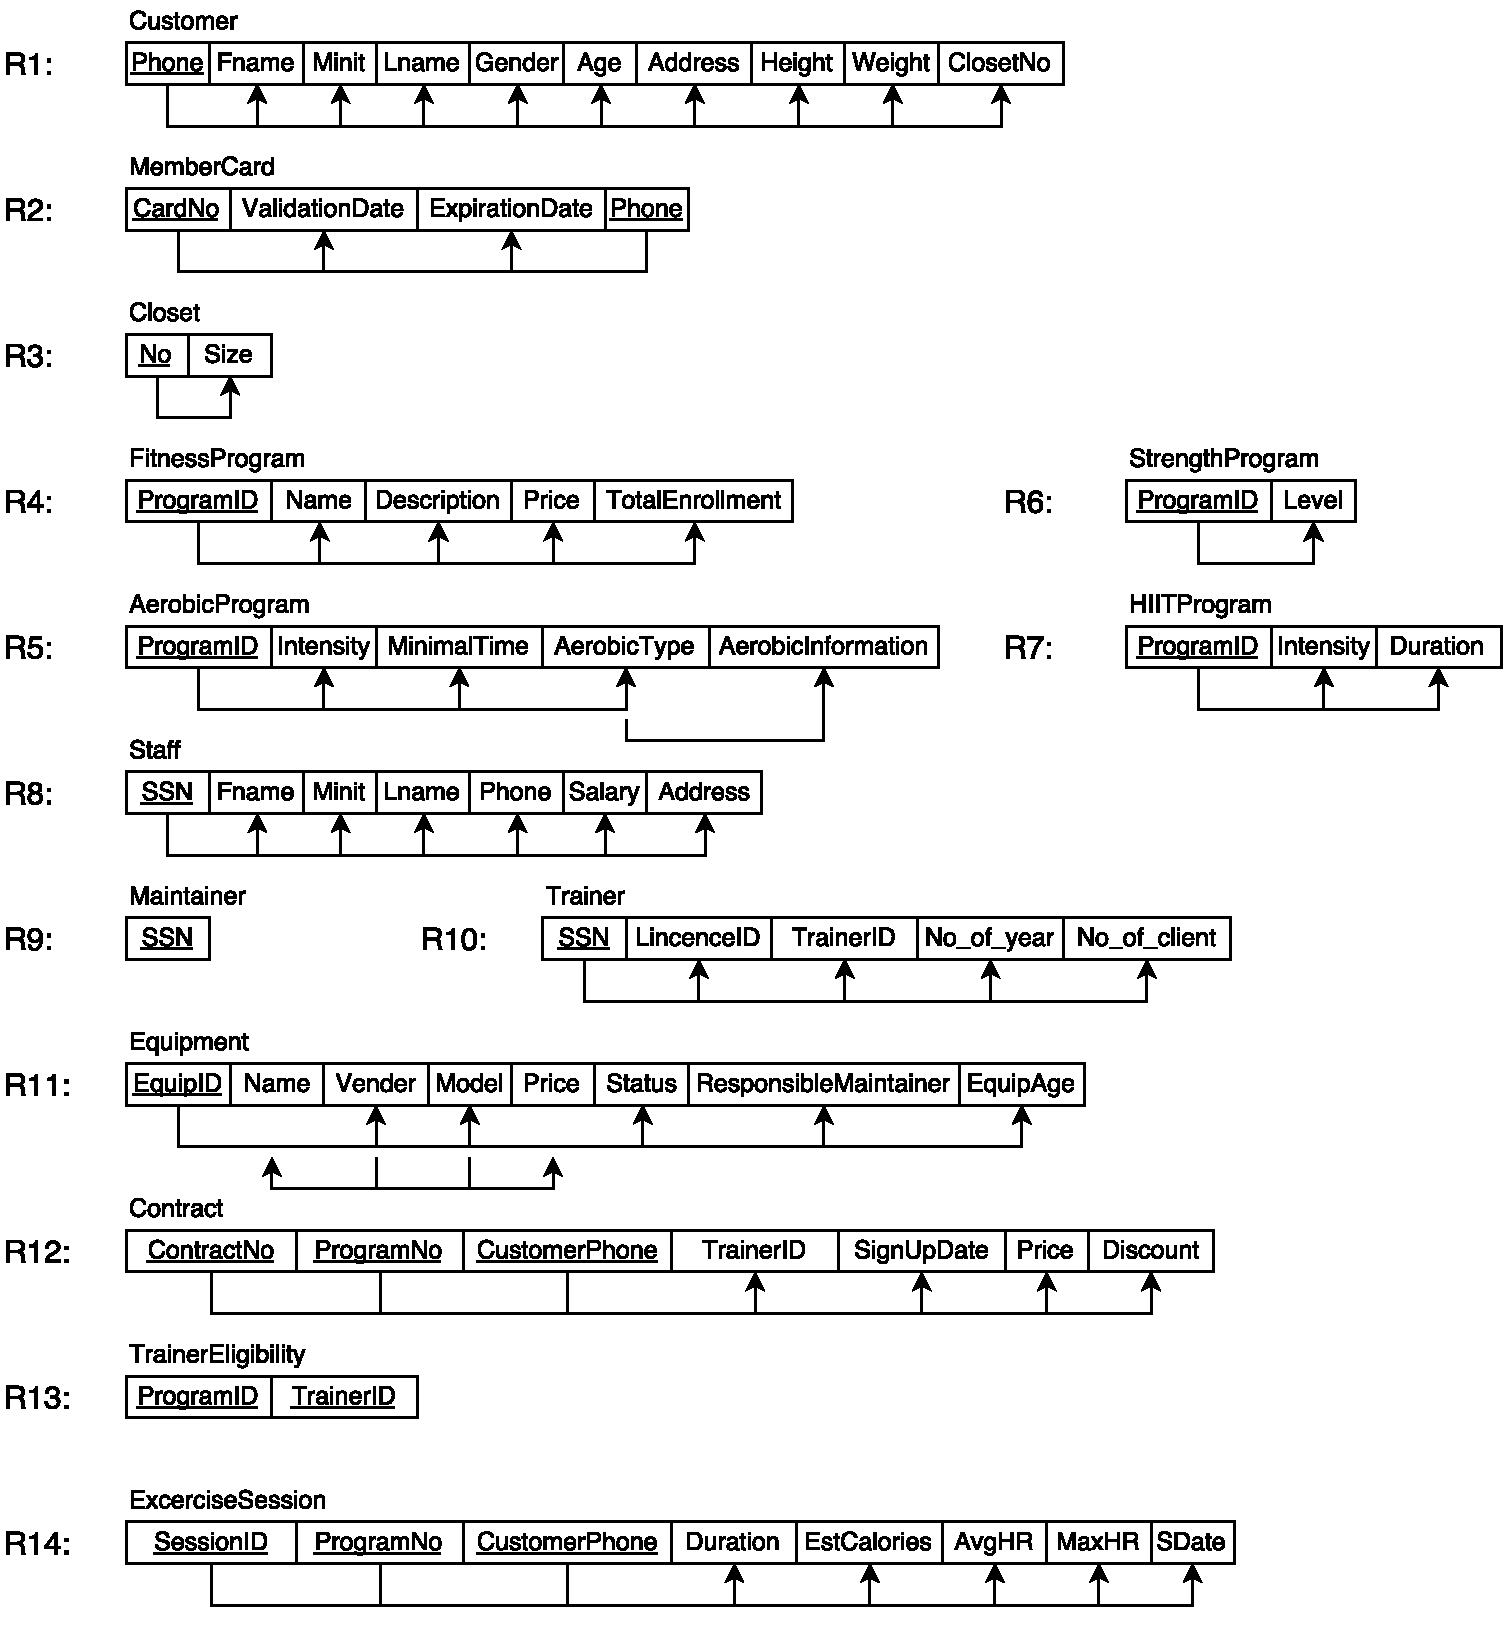
\includegraphics[width=\textwidth]{img/fd}
\end{figure}

We can see from \cref{fd} that $R5$ and $R11$ violates 3NF.
To normalize these relations, we need to remove the transitive functional dependencies in the relation.
The normalization process is shown in \cref{norm}, $R5a$, $R5b$ substitute the original $R5$, $R11a$ and $R11b$ substitute the original $R11$.
\begin{figure}[H]
    \caption{Normalization Process}\label{norm}
    \centering
    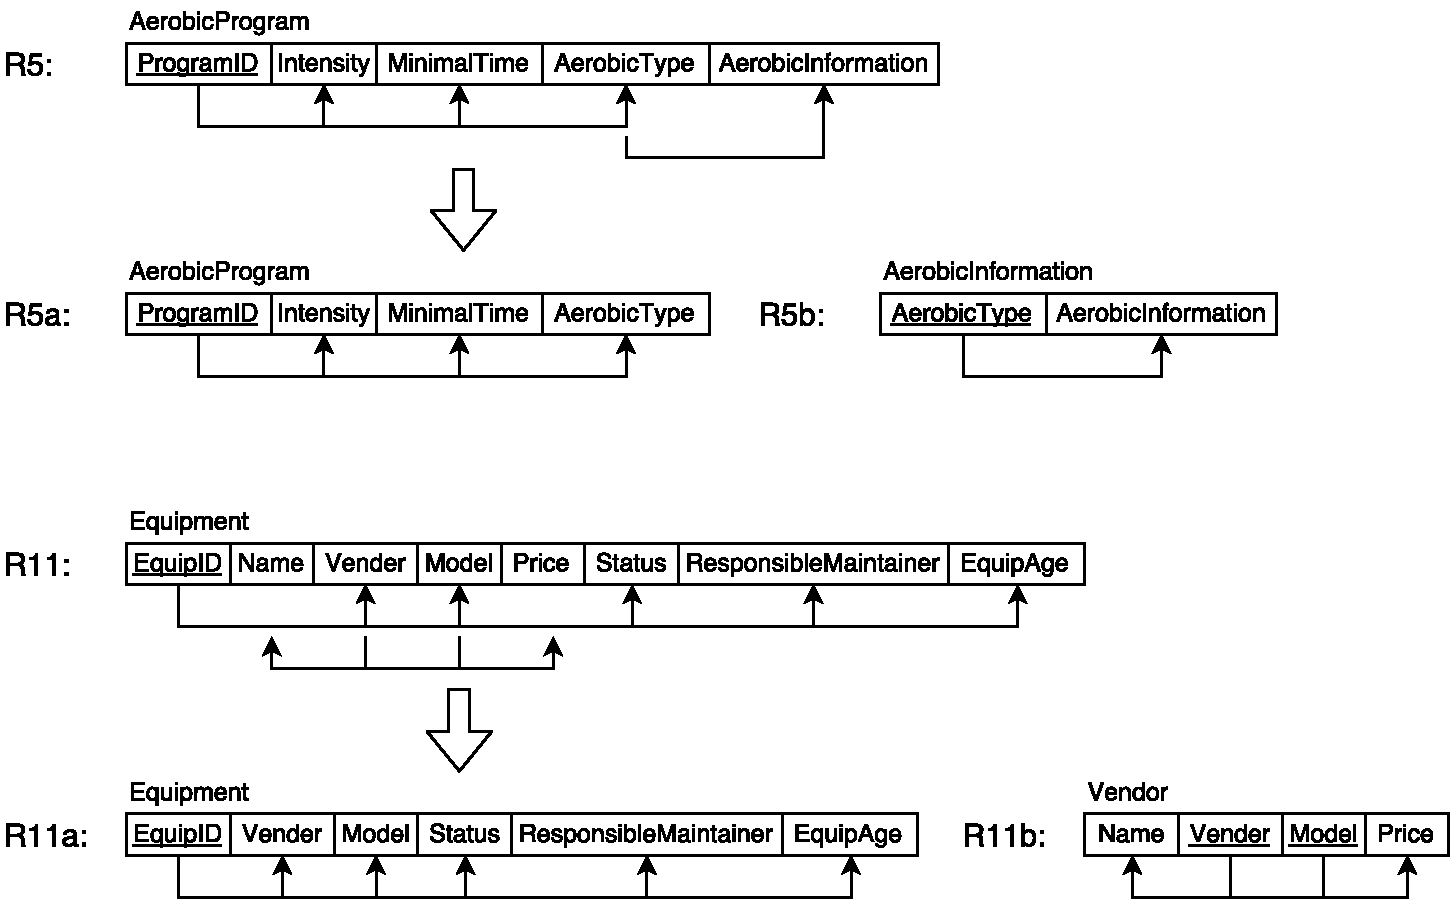
\includegraphics[width=\textwidth]{img/norm}
\end{figure}

\section{SQL}
The \texttt{CREATE} table command is as follow.
\lstinputlisting[style=customSQL]{src/createTable.sql}

\section{Trigger}
\subsection{Update Total Enrollment of Program}
Each time a record was added to the \textsc{Contract} table,
the $TotalEnrollment$ in table \textsc{FitnessProgram} of the particular program should add 1.

The trigger is defined as follow:
\lstinputlisting[style=customSQL]{src/addTotalEnrollmentTrigger.sql}

\subsection{Log all the changes about Customer}
Each time a record was added/updated/deleted in \textsc{Customer} table,
record the modification in \textsc{Customer\_Log} table.

The trigger is defined as follow:
\lstinputlisting[style=customSQL]{src/customerLogTrigger.sql}

\section{Procedure}

\subsection{Delete old Exercise Session Data for Customer}
According to requirement, the database should only keep exercise session data
of non-member customer for two years, three for customer with expired membership,
and forever for current member. Therefore, there would be a circumstance that
we want to delete exercise session data of two years old for customer without member,
as well as the exercise session of three years old for customer with expired member card.
The procedure is defined as follow:
\lstinputlisting[style=customSQL]{src/deleteSessionOfIdleCustomer.sql}

\subsection{Add Bonus for Specific Member}
Assume a deal event want to add some bonus time for member registered during specific period.
The procedure is defined as follow:
\lstinputlisting[style=customSQL]{src/addBonusTimeProcedure.sql}
\section{Business Rule}
\subsection{Check the Age of the Equipment}
Assume not allowing a equipment older than 5 years, the constraint is defined as follow:
\lstinputlisting[style=customSQL]{src/checkEquipAge.sql}

\subsection{Check the TotalEnrollment of a Fitness Program}
Assume not allowing a fitness program's total enrollment shall not exceed 50,
the constraint is defined as follow:
\lstinputlisting[style=customSQL]{src/checkTotalEnrollment.sql}

\subsection{Check the Number of client of a Fitness Trainer}
Assume not allowing a fitness trainer's client number shall not exceed 50,
the constraint is defined as follow:
\lstinputlisting[style=customSQL]{src/checkNo_of_clients.sql}

\section{Appendix}
Here is some sample data.
\lstinputlisting[style=customSQL]{src/sampleData.sql}

\end{document}
